\chapter{Implementation}

\label{ch:Implementation} 

\lhead{Kapitel 3. \emph{Implementation}}

\section{Programmeringsspråk}

Under den inledande fasen av projektet hade vi livliga diskussioner om vilket programmeringsspråk vi skulle använda. Vi bestämde att projektet skulle kretsa kring actor-modellen, det satte begränsningar på vilka språk vi kunde använda. Vi funderade först på att använda något nyutvecklat experimentellt språk och det stod mellan Nim och Rust. Efter mycket diskussion så skrotade vi denna idé då Nim\footnote{\url{http://nim-lang.org/}} är ett mycket nytt och instabilt språk, samtidigt som Rust\footnote{\url{http://www.rust-lang.org/}} är ett för strikt och invecklat språk. Användandet av Rust hade lett till att vi hade fått spendera mycket tid på lärandet av språket istället för att fokusera på de mer väsentliga delarna av projektet. 

Vi valde istället att använda Erlang för då det är ett väletablerat och stabilt språk byggt kring actor-modellen och message-passing. Utöver Erlang använde vi Python för den grafiska delen och ErlPort\footnote{\url{http://erlport.org/}} för kommunikationen mellan Erlang och Python. Implementationen av ErlPort har fungerat mycket bra och har gett oss ett smidigt interface mellan Erlang och Python.

\section{GUI}

GUI-modulen initieras med att skapa en lista motsvarande hela griden, den fylls med tomma atomer som Python-modulen inte ritar ut. GUI-modulen körs i en main loop som tar emot meddelanden från cell-modulerna, bearbetar dessa och fyller på den initierade listan. 

En algoritm används för att fördela listan på rätt X och Y koordinater, koordinaterna är angivna i meddelandet från cellen. Listan skickas via ErlPort till Python där den ritas upp grafiskt.

\subsection{Erlport}

Erlport är ett bibliotek som gör det möjligt för Erlang att kommunicera med andra programmeringsspråk. I dagsläget har Erlport stöd för Python och Ruby. 

För att Erlport ska kunna kommunicera med Python så skapar man först en instans, en Python instans är i princip en OS-process som representeras i Erlang av en Erlang process. Man kan skicka och ta emot medelanden mellan Erlang och Python på samma sätt som man skickar meddelanden mellan vanliga processer i Erlang.

\subsection{Pygame}

För den grafiska renderingen i projektet har vi använt oss av det community-utvecklade Pythonbiblioteket Pygame. Pygame är ett bibliotek av färdigutvecklade moduler till Python designade för att enkelt kunna skapa spel med en enkel grafisk implementation. Pygames design gör att det är enkelt att använda på alla plattformar som har stöd för Python.

\section{Ants and Cells}

Ant-modulen och Cell-modulen är väldigt lika varandra i sin implementation. Båda modulerna består utav en initialiseringsfunktion som används för att starta processer. Funktionen inväntar de meddelanden som är nödvändiga för att starta processerna. Detta kan till exempel vara ett meddelande om att myran har placerats korrekt och att cellerna har fått sitt grannskap definierat.

Cellerna och myrorna går efter ett meddelande till sin mainfunktion där de inväntar nya förfrågningar. Om det inte finns några obehandlade meddelanden kommer myrorna att agera spontant. När cellerna och myrorna får ett inkommande meddelande kommer de att anropa en funktion specifikt för den typen av meddelande. Dessa funktioner kan skicka och ta emot meddelanden själva med hjälp av meddelandefiltreringen. När en förfrågan eller annat meddelande har behandlats kommer processen återgå till sin mainfunktion. Om ett felaktigt eller otillåtet meddelande inkommer under någon del av exekveringen så kommer hela systemet att krascha.

Cellerna kommer vid varje inkommen förfrågan, beroende av cellens tillstånd, automatiskt genomföra en uppdatering av dess feromonnivåer. Detta sker som en funktion av den faktiska tiden(wall-time) som har gått sedan cellen senast uppdaterades.

Om en cell har attributet  \emph{block} så kan en myra inte gå dit och alla \verb+place_ant+ förfrågningar kommer att misslyckas.

\subsection{Myrans algoritm}

Myran beslut baseras på en väldigt enkel algoritm. Myran kan vara i två olika tillstånd \verb+searching_for_food+ och \verb+returning_with_food+. 

När myran letar efter mat så kommer den att undersöka cellen den står i, om det finns mat i cellen så kommer myran att försöka plocka upp maten. Om myran lyckas plocka upp mat kommer den att byta tillstånd till \verb+returning_with_food+, om myran misslyckas med att plocka upp mat så kommer den att fortsätta leta efter mat i andra celler.

När myran letar efter mat så kommer den att be cellen den står i att skicka tillbaka information om alla celler i dess grannskap. Myran kommer sedan att studera sitt grannskap och sortera cellerna efter hur mycket \verb+food_feremone+ varje cell innehåller och sedan genom \emph{rank-selection} att välja den riktingen den skall gå i. Rank-selection innebär att den med en förutbestämd sannolikhet $p$ kommer att gå till den cellen med det högsta antalet feromoner. Om den inte väljer den riktningen så kommer den att gå till den cellen med näst högst riktning med samma sannolikhet $p$.

Myran kommer efter varje genomförd förflyttning att släppa feromoner på den cellen där den tidigare var. Då myran letar efter mat kommer den att släppa \verb+base_feremone+ och då den går tillbaka med maten så kommer den att släppa \verb+food_feremone+.

Då myran går tillbaka med mat så kommer den att följa en snarlik algoritm men istället leta efter den högsta koncentrationen utav \verb+base_feremone+.

I figur \ref{fig:myralgo} finns en flow-chart om hur algoritmen ser ut.


\begin{figure}
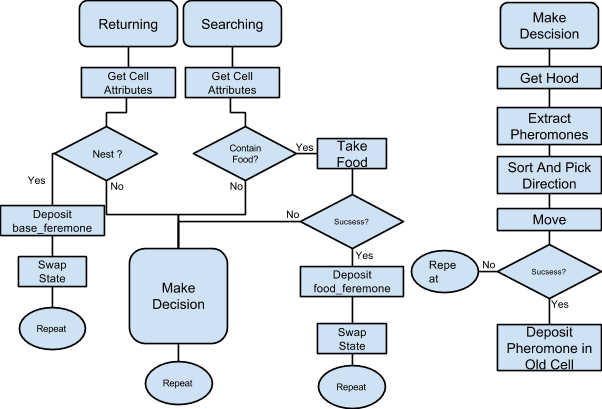
\includegraphics[scale=0.6]{Figures/myralgo.png}
\caption{Flowchart över myrans algoritm}
\label{fig:myralgo}
\end{figure}

\subsection{Grid\_Init}

Grid\_init är den modul som bygger upp världen. Det första som den modulen gör är att den startar alla cell-processer. Det krävs att GUI-modulen är startad, dess PID kommer att skickas med till alla celler. Den kommer sedan att skicka ut \verb+set_cell_attribute+ medelanden till alla dessa celler med cellernas attribut. Grid\_init kommer sedan att initiera en \emph{Queen}\footnote{Queen processen samlar in statistik från myrorna och används endast för debugging och testning.} process och starta alla myror och försöka placera ut dem på de celler där de skall starta. När alla myror har blivit utplacerade så kommer Grid\_init modulen att skicka \verb+start_ant+ medelanden till myrorna vilket kommer att starta simuleringen.

\section{Concurrency}

Då concurrencyn i vårat program uteslutande bygger på actor-modellen och message passing så har vi definierat tre klasser utav meddelanden.

\begin{itemize}

\item One-way meddelanden är på formen \verb+{Pid,{Type,Payload}}+ eller \verb+{Pid,Type}+
	One-way meddelanden är meddelanden som inte kommer att resultera i att något svar inkommer.

\item	Request (förfrågningar) meddelanden är på formen \verb+{Pid,Reference,Payload}+
	Alla Request-meddelanden resulterar i att processen blockerar och inväntar Reply-meddelanden.

\item	Reply-meddelanden är på formen \verb+{Pid,Refernce,Request_Reference,{Type,Reply_Payload}}+
	Reply-meddelanden är de meddelanden som skickas som svar på requests.

\end{itemize}


I alla meddelanden så är \verb+Pid+ att vara process id:t hos processen som skickar meddelandet \verb+Payload+ är vad meddelandet faktiskt innehåller  \verb+Reference+ är den referens som den skickade processen ger meddelandet \verb+Request_Reference+ är den referensen från ett request meddelande till vilket detta är ett svar.

Då systemet faller under \emph{ asynchronous event-driven programming} så kan vissa problem uppstå om vi inte är försiktiga med hur vi implementerar systemet. Det naiva tillvägagångssättet hade varit en så kallad \emph{Fifo, run to completion} metod. Detta innebär att man accepterar varje meddelande, hanterar det och låter det köra tills det att det är klart innan man hanterar nästa meddelande. Fifo-metoden leder dock till problem med att man måste hålla explicit koll på vilket tillstånd processen är i och ha en plan för hur man ska hantera alla kombinationer av meddelande-tillstånd. Detta skulle ha lett till extremt komplicerad och svårhanterlig kod.\citep{Reference5}

Lösningen på detta är att använda vad vi kallar för \emph{state-driven message handling}, vilket är att vi låter en process tillstånd diktera vilka meddelanden som den kommer att hantera. Det vi gör är att vi implementerar ett meddelandefilter som bara returnerar rätt meddelande (baserat på meddelandets unika tag/referens) och alla andra meddelanden som inkommer läggs på en buffer så att de senare kan hanteras.

Detta leder till att koden blir kortare och lättare att underhålla då vi på ett lätt sätt kan hantera hur systemet beter sig. Det finns dock ett krav på att alla processer måste ha ett eller flera tillstånd då de accepterar nya meddelanden. I detta tillstånd kommer meddelanden som ligger på buffern att hanteras först och när buffern är tom kommer de nya meddelandena att hanteras.


\subsection{Deadlocks}


Vår simulering är full av deadlocks och de uppstår ofta. Vi är därför tvungna att ha något system för att upptäcka och lösa alla deadlocks.

Vi kan för enklare deadlocks lösa detta effektivt och deterministiskt. Vi vet att om en process väntar på svar på en förfrågan så kommer den att blockera. Om en process väntar på ett svar från en annan process men får en förfrågan från den processen innan den har fått svar så vet vi att ett deadlock har uppstått. Processen som upptäcker att ett deadlock har uppstått kommer direkt att ge svar om misslyckande till den förfrågan som orsakade deadlocken. Det leder till att den andra processen kommer sluta blockera och förfrågan kan därefter hanteras. Detta förutsätter att det alltid är tillåtet för en förfrågan att misslyckas och att en process alltid kommer efter en finit tid kunna hantera nya förfrågningar efter det att en förfrågan har misslyckats.

Den här metoden kan bara endast lösa deadlocks som uppstår mellan två processer, men vi drabbas ständigt av mer komplicerade deadlocks i systemet.

Vi har konstruerat en metod för att lösa mer komplicerade distribuerade deadlocks som är väldigt simpel men mycket effektiv. Vår metod löser alla deadlocks helt automatiskt och kräver inte att några rollbacks \footnote{Att systemet återställs till ett tidigare tillstånd} måste genomföras eller analys av det globala tillståndet med en Wait-For-Graph.\citep{Reference6} Vår metod kräver inte heller att några \emph{probe} meddelanden skickas mellan processerana som i Chandy-Misra-Haas algoritmen.\citep{Reference7}

Dock så predikeras vår metod på en uppsättning krav på systemet.

\begin{itemize}
\item Alla förfrågningar kan misslyckas på ett väldefinierat sätt.

\item Alla processer kommer att invänta ett svar efter en förfrågan har skickats. 

\item Från det att ett svar på en förfrågan har inkommit kommer processen alltid att inom en finit tid drivas till ett tillstånd där den accepterar inkommande förfrågningar.
\end{itemize}

Dessa är en uppsättning preliminära predikat. Det kan finnas ytterligare begränsningar som vi har missat då de inte är applicerbara på vårt system. Även då dessa predikat kan förefalla vara hårda så innebär inte det att funktionaliteten drabbas signifikant. De tillåter att en process som väntar på ett svar fortfarande kan hantera vissa meddelanden och skicka nya förfrågningar till processer. De tillåter även att man implementerar en prioritering utav olika typer av förfrågningar eller olika typer av processer.

När en process väntar på svar från en annan process så kommer den att efter en viss förutbestämd tid (timeout), skicka automatiska fail-svar till alla inkomna förfrågningar som ligger på dess meddelande-buffer. Detta kommer att repeteras tills att ett svar har inkommit. Ni kan se en schematisk beskrivning av algoritmen i figur \ref{fig:receiver}.

\begin{figure}
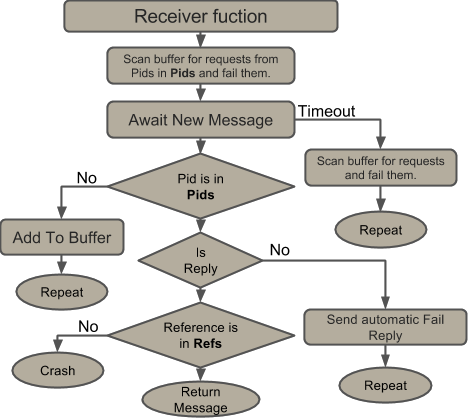
\includegraphics[scale=0.8]{Figures/receiver.png}
\caption{En schematisk överblick över hur meddelandefiltreringen och deadlock-hanteringen fungerar. \textbf{Refs} är en lista med de referenser från de förfrågningar meddelanden som har skickats.  \textbf{Pids} är en lista med de Pids som förfrågningarna har skickats till.}
\label{fig:receiver}
\end{figure}

Vår metod har dock den nackdelen att den ofta kommer att upptäcka \emph{falska deadlocks}, det vill säga att den kommer att tro att det finns ett deadlock när det inte gör det och i onödan avvisa vissa förfrågningar. Detta leder till att \textbf{Timeout} parametern måste finjusteras. En timeout som är för lång kommer innebära att deadlocks kommer att ligga kvar för länge innan de upptäcks och delar utav simuleringen kommer att  \emph{lagga}. En för kort timeout kommer att leda till att väldigt många förfrågningar kommer att avisas i onödan vilket också kan påverka systemets prestanda.
























